\chapter{Hyperparameter Tuning}
Many machine learning algorithms have one or more hyperparameters, whose role is to modify different aspects of the learning process. Their values are not estimated through use of the training data, but must be chosen prior to the start of the learning process. Choosing a set of suitable hyperparameter values for a learning algorithm, also called model selection, is an important step to ensure that the algorithm performs well and does not overfit the training data.

\section{Traditional approaches}

\subsubsection{Grid Search}
Grid search, also called parameter sweep, is commonly used to perform hyperparameter optimization. A predefined set of values is selected for each of the tuning parameters used by the learning algorithm. Models are then trained with each possible combination of tuning parameter values. All models are evaluated according to some performance metric. The combination of parameter values that produces the model performing best (minimizing/maximizing the performance metric) is chosen as optimal. The performance metric used typically in regression problems is the mean squared prediction error (MSE), calculated as shown in Equation \ref{eq:mse}.
\begin{equation} \label{eq:mse}
MSE = \frac{1}{n} \sum_{i=1}^{n} (\hat{y_i}-y_i)^2, 
\end{equation}
where $\hat{y_i}$ is the model's predicted value and $y_i$ is the true value of the target. 

\subsubsection{The Validation Set Approach}
Estimating a model's MSE using the same data it was trained on is not truly indicative of the model's performance due to the possibility of overfitting. One way to measure a model's accuracy of prediction on unseen data is to calculate generalization error, also known as out-of-sample error. 

This could be done through the validation set approach by partitioning the available data into two mutually exclusive subsets called training and test (validation) sets. Models are then trained on the training subset of observations and their prediction MSE is calculated using the test set, also called holdout. However, this method has the following drawbacks \cite{james2013introduction}:
\begin{itemize}
	\item The validation estimate of the test error rate can vary greatly depending on the training-validation set partitioning
	\item The method makes inefficient use of the data as a significant part of the observations are never used for training
\end{itemize} 

\subsubsection{K-Fold Cross Validation}
Cross validation \cite{james2013introduction, kohavi1995study} is a resampling method closely related to and addressing the drawbacks of the validation set approach. The often used k-fold cross-validation involves partitioning the data into $k$ subsets (folds). One of the folds is treated as a validation set and the model is trained on the remaining $k-1$ folds. The mean squared error for the fold $MSE_i$ is computed for the observations in the held-out fold $i$. The process is repeated $k$ times, each of the folds being held out once, and the k-fold CV estimate is obtained by averaging the estimates for the different folds as shown in Equation \ref{eq:cv}.
\begin{equation} \label{eq:cv}
MSE_{(k)} = \frac{1}{k} \sum_{i=1}^{k} MSE_i
\end{equation}

\subsubsection{Grid Search minimizing the Cross-Validated MSE}
One traditional approach of performing model selection uses a grid search with cross-validated mean squared prediction error for a metric of model performance. The final model is then trained on the whole dataset using the optimal hyperparameter values that minimize the cross-validated MSE. This model selection approach is denoted as "CV-MSE" tuning in the latter chapters of this report.

\section{Orchestrated Parameter Tuning}

\subsection{Context and motivation}
In the context of this project multiple methods of performing regression are defined, each of them minimizing a different objective function. All approaches operate on the same training data and share a common goal to correctly identify the relationship between predictors and the target variable. 

Traditionally, we would tune the hyperparameters for each regression method independently before processing the desired data with the optimal parameter combinations for each method. Such an approach would not benefit from having an ensemble of regression approaches as they would all function completely independently. Our aim was to develop a hyperparameter optimization approach that would use this presence of multiple alternative approaches to perform simultaneous and cooperative parameter tuning.

\subsection{Inspiration}
Our novel hyperparameter tuning approach presented in Section \ref{sec:orc_meth} is inspired by a different kind of ensemble, that of a philharmonic orchestra. Much like the different regression methods, every musical instrument produces its own distinguishing sound even when playing the same melody. All of the various instruments complement each other and contribute in their own way to the skillful masterpiece that is a symphony. 

During a performance every musician needs to ensure that they are in synchronization with the rest of the orchestra. They need to be constantly aware of what the current general tempo and state of the melody across the whole ensemble is. In case of a mismatch, the performer needs to adjust their own way of playing their instrument to bring it back to synchronization with the other instruments.

The behavior of each regression method in our proposed hyperparameter tuning closely resembles these synchronizing adjustments made by orchestra members during a performance.

\subsection{Methodology} \label{sec:orc_meth}
We propose an alternative approach for simultaneous cooperative hyperparameter tuning that uses an ensemble of regression methods sharing a similar goal and input data. Our tuning method features an iterative algorithm that attempts to increase the similarity between parameter estimates of the various regression approaches at each step.

\subsubsection{Iterative procedure}
Initially, each of the methods is trained using some hyperparameter combination in their respective search grids, forming the method outputs for the "zero" iteration. The choice of this initial starting point is discussed in a subsection below.

\begin{figure}[H]
	\centering
	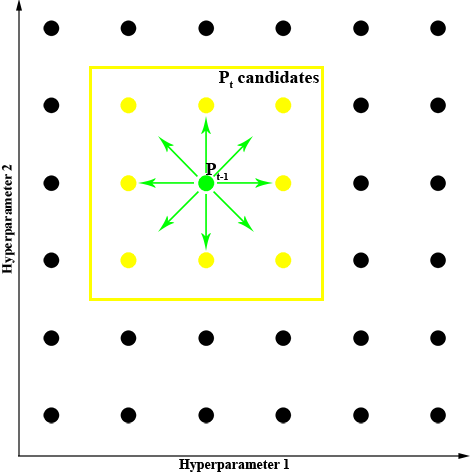
\includegraphics[scale=0.66]{search_grid}
	\caption{Local search grid neighborhood, two tuning hyperparameters; $P_{t-1}$ is the parameter combination selected in iteration $t-1$, parameter values in the $P_t$ neighborhood are considered in iteration $t$}
	\label{fig:orc_tun_search_grid}
\end{figure}

The orchestrated tuning procedure for each method $M$ in iteration $t$ is defined as follows:
\begin{enumerate}
	\item \label{target_vector} Consider the coefficient vectors estimated by all other methods for the previous iteration. A target coefficient vector is calculated by averaging the estimated parameters of all other methods.
	\item \label{cand_comb} Consider the candidate hyperparameter value combinations located in proximity (in the search grid) to the combination selected by the previous iteration. An example of a set of candidate combinations is shown on Figure \ref{fig:orc_tun_search_grid} for a regression method with two tuning parameters. Train the regression method with each of the candidate combinations.
	\item Consider the estimated coefficient vectors resulting from each of the candidate parameter combinations. The hyperparameter combination chosen for the current iteration is the one that maximizes correlation between its estimated vector and the target vector defined in \ref{target_vector}. The method's estimate for the current iteration is the one produced by the chosen candidate combination.
\end{enumerate}

\begin{figure}[bh]
	\centering
	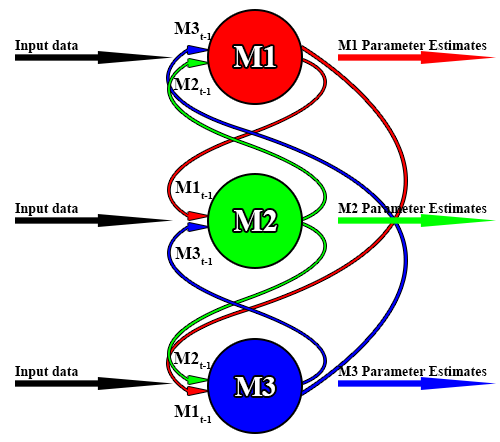
\includegraphics[scale=0.75]{orchestrated_tuning_methodology}
	\caption{Orchestrated tuning abstract structure, three regression methods; $M1_{t-1}$ denotes the parameter estimates of method $1$ for iteration $t-1$; Each tuning iteration $t$ of a method uses the common input data and the parameter estimates of all other methods for the previous iteration}
	\label{fig:orc_tun_struct}
\end{figure}

This iterative procedure converges when any movement along the parameter grids is settled for all methods. The tuning stops when the selected hyperparameter combinations for the current iteration are identical to those of the previous iteration for all methods. The combination of parameter values for each method selected by the last iteration is considered optimal.

If the parameter search grids for the various methods are coarse, fluctuation between two parameter combinations can occur preventing convergence. A maximum number of iterations can be defined to force the completion of the tuning process, resulting in an approximate solution. 

\subsubsection{Choice of starting points for the search}
%Initially, each of the methods is trained using the median value of each of its parameters (that is, if the considered values are lambda1= [0.05, 0.1, 1, 10, 20] and lambda2 = [0.1, 0.2, 0.3, 0.4, 0.5], values lambda1=0.1 and lambda2=0.3 will be used) 

\subsubsection{Discussion}
%Such a parameter tuning process finds such values for the various methods' parameters that lead to the production of similar coefficient vectors across methods. As explained earlier, the focus is on the predictor coefficients that are estimated in each iteration and not on the prediction error, this is why cross validation is not needed and the parameter tuning process is optimized in terms of computing power. What is more, it uses the fact that we have multiple methods and they perform their parameter tuning cooperatively so as to ensure consensus across methods after the training with arbitrary data.



